\documentclass[conference]{IEEEtran}
\IEEEoverridecommandlockouts
\usepackage{cite}
\usepackage{amsmath,amssymb,amsfonts}
\usepackage{graphicx}
\usepackage{textcomp}
\usepackage{xcolor}
\usepackage{subfigure}
\usepackage{subcaption}
\usepackage{hyperref} % immer als letztes!
\renewcommand{\citepunct}{,\penalty\citepunctpenalty\,}

\begin{document}
%Vorher wurde von mir das falsche Template leider genutzt
\title{In Tune with the Room: Advancing Blind RIR Generation
Through a Comprehensive Evaluation Framework}

\author{
\IEEEauthorblockN{Sebastian Stauß$^{1,2,3}$, \; Hiroshi Watanabe$^{3}$, \; Thomas Schmid$^{1,4,5,6,7}$}
\IEEEauthorblockA{
\footnotesize
$^{1}$ Medical Faculty, Martin Luther University Halle-Wittenberg, Halle, Germany \quad
$^{2}$ Institute of Computer Science, Leipzig University, Leipzig, Germany \\
$^{3}$ Graduate School of FSE, Waseda University, Tokyo, Japan \quad
$^{4}$ Institute of Computer Science, Martin Luther University Halle-Wittenberg, Halle, Germany \\
$^{5}$ Research Center Data Analytics, University Hospital Halle, Halle, Germany \quad
$^{6}$ Data Science \& AI Institute, Lancaster University, Lancaster, United Kingdom \\
$^{7}$ School of Computing and Communications, Lancaster University Leipzig, Germany \\
}
}
\maketitle

\begin{abstract}
Room Impulse Responses (RIRs) model how sound interacts with acoustic environments and are critical for virtual reality, sound design, and related applications. Accurate RIR generation is therefore essential, yet existing evaluation approaches remain fragmented, relying on different datasets and metric combinations that capture only limited aspects of RIR characteristics. In addition, most current models are not publicly available, further hindering direct comparison. We introduce a comprehensive multi-metric framework combining metrics including DRR, T60, energy decay relief (EDR), multi-resolution STFT loss (MSTFT loss), and a newly designed peak similarity metric quantifying spectral peak accuracy. Using this framework, we compare two alternative enhancements to a popular deep learning approach for blind RIR generation: the Filtered Noise Shaping (FiNS) architecture. In the first approach, we optimize filterbank initialization by deriving center frequencies from statistical analysis. In an alternative approach, we combine MSTFT loss with EDR loss to improve spectral details and frequency-dependent energy decay patterns. Evaluation on 11,500 RIRs from 295 rooms across 11 datasets demonstrates substantial improvements for the loss-based approach: 41\% reduction in MSTFT loss, 25\% increase in peak similarity, and superior frequency-dependent energy decay modeling.
\end{abstract}
 
\begin{IEEEkeywords}
room impulse response, machine learning, acoustic modeling, audio processing, blind estimation
\end{IEEEkeywords}
 
\section{Introduction}
 
%Room acoustics significantly impact human health and wellbeing, with people spending the majority of their time in indoor environments where acoustic properties directly influence comfort and communication effectiveness \cite{NAEEMAEE2024comfort,WHO2018noise}.
Room impulse responses (RIRs) characterize the acoustic transfer function of a space, encoding how sound propagates from source to receiver through direct paths, early reflections, and late reverberation \cite{kuttruff2016room}. Accurate RIR modeling is critical for many applications, including speech enhancement \cite{ratnarajah2023towards} and virtual reality audio \cite{lee2023yet}. Traditionally, RIR acquisition requires specialized equipment, controlled conditions, and significant time investment \cite{szoke2019building}. This has motivated the development of blind estimation methods that predict RIRs directly from reverberant audio signals \cite{steinmetz2021filtered, ratnarajah2023towards, lee2023yet, lee2023RIRmultiple, Lin2024deeproomimpulseresponse, lin2006bayesian, crammer2006room}. 
 
Classical blind estimation approaches using deconvolution and statistical methods \cite{lin2006bayesian, crammer2006room} have been largely superseded by deep learning techniques. Recent approaches include Generative Adversarial Networks \cite{ratnarajah2023towards}, Variational Autoencoders \cite{lee2023yet}, and the Filtered Noise Shaping (FiNS) model \cite{steinmetz2021filtered}. FiNS has emerged as an effective tool due to its physically motivated architecture separating direct sound with early reflections from late reverberation using trainable filterbanks to shape noise for realistic late reverberation synthesis. However, listening tests reveal that synthetic RIRs generated by FiNS can still be distinguished from measurements \cite{steinmetz2021filtered}. Quantifying such perceptual differences remains challenging, since conventional metrics capture only limited aspects of the RIR. FiNS, despite being introduced in 2021, continues to serve as a standard baseline for blind RIR estimation (\cite{ratnarajah2023towards, saini2024EDC, lee2023yet}) and has spawned several recent modifications (\cite{Lin2024deeproomimpulseresponse, lee2023RIRmultiple}). 
 
%Our main contributions include: (i) a comprehensive evaluation framework for RIR generation, (ii) a robust MSTFT+EDR loss function combination, (iii) a novel peak similarity metric for evaluating spectral peak accuracy.
 
\section{Related Work}
 
RIR estimation approaches span from multimodal methods to pure audio-based blind estimation. Multimodal methods leverage visual information including images \cite{chen2022imageRIR,nikhil2021image2RIR}, videos \cite{garg2021videoRIR,liang2023avnerfVid2RIR}, or 3D room models \cite{tang2020model3dgraphics}. While promising, these require additional sensors or complex 3D modeling, limiting practical deployment. Simplified variants using floor plans \cite{lundin2022grundriss} or feature maps \cite{falcon2021featureMaps} reduce complexity but remain constrained by geometric information requirements.
 
In contrast, blind RIR estimation requires only audio signals. Neural RIR generation has evolved from classical parameter estimation \cite{gamper2018blind, looney2020} to  generative models that synthesize complete impulse responses directly from reverberant audio \cite{steinmetz2021filtered, ratnarajah2023towards, lee2023yet}. Early classical methods \cite{lin2006bayesian, crammer2006room} employed statistical techniques but required specific signal types or multi-channel recordings, limiting applicability. The ACE Challenge \cite{eaton2016estimationACE} established benchmarks for T60 and DRR estimation, motivating ML-based approaches. Later, parameter estimation methods \cite{gamper2018blind, looney2020, bryan2020impulse, gotz2022} achieved improved accuracy but remained limited to parameter extraction rather than RIR synthesis. Saini and Peissig \cite{saini2024EDC} recently demonstrated superior EDC/EDR estimation using GANs, achieving T60 MSE of 0.01s.
 
Modern RIR generation employs diverse neural architectures. The S2IR-GAN \cite{ratnarajah2023towards} uses adversarial training with EDR loss, achieving 17\% EDR improvement over FiNS but limited to 16kHz sampling with 0.25s RIRs. Lee et al. \cite{lee2023yet} proposed a two-stage approach using VAEs for token-based RIR representation with autoregressive Transformer decoding, effective for acoustic matching but computationally expensive with performance degradation for T60 $>$ 0.7s. 
 
Due to limited code availability, recent approaches primarily compare against FiNS using selected metrics and individual datasets, which makes cross-method comparison difficult and less reliable. Known limitations of FiNS in spectral accuracy remain. Here, we investigate two complementary strategies to address these limitations: (a) an improved FiNS filterbank design and (b) combined loss functions. These enhancements also serve to demonstrate the proposed evaluation framework.
 
\section{Proposed Evaluation Framework} 
 
%We propose using a representative multi-faceted dataset for the evaluation of RIR generation and employing a combination of ten different metrics\footnote{https://github.com/AIIM-Group/RIRBench}, which allows for convenient interpretation using a radar plot (see Figure \ref{fig:radar-all}) in addition to an EDR table for detailed core frequency band analysis.

We propose using a representative multi-faceted dataset for the evaluation of RIR generation and employing a combination of ten different metrics, which allows for convenient interpretation using a radar plot (see Figure \ref{fig:radar-all}) in addition to an EDR table for detailed core frequency band analysis.\footnote{Code and dataset links: \url{https://github.com/AIIM-Group/RIRBench}}
 
\subsection{Data}
We combine 11 RIR datasets, totaling 11,500 RIRs from 295 rooms across 11 datasets: R3VIVAL \cite{klein2023r3vival}, Arni \cite{Prawda2022ArniDataset}, Palimpsest \cite{pasoulas2022palimpa}, BBC Maida Vale \cite{kearney2022BBC}, Motus \cite{Gotz2021MotusDatasetPaper}, Detmold-SRIR \cite{amengual2020Detmold}, MIT IR Survey \cite{traer2016MIT}, ACE Challenge \cite{eaton2016estimationACE}, C4DM RIR \cite{stewart2010c4dm}, AIR \cite{murphy2010openair}, and MYRiAD V2 \cite{dietzen2023myriad}. Speech data comprises 44,455 VCTK \cite{yamagishi2019vctk} utterances from 110 speakers. Data is split 60/20/20 for training/validation/test with proportional representation across all splits.
 
\textbf{Processing.} Amplitudes of all RIRs are normalized to 0.9 peak, initial delays removed through energy-based onset detection, resampled to 48kHz using polyphase method, truncated to 1-second with 50ms linear fadeout, and converted to mono (first channel; left for stereo, W-component for B-format). The Arni dataset was subsampled from 132k to 3.5k RIRs based on acoustic panel configuration diversity.
 
 
\subsection{Metrics}

In order to achieve a comprehensive evaluation of blind RIR generation, we combine metrics for spectral accuracy, temporal energy modeling, and robustness.

\textbf{T60} (bias, MSE, correlation) quantifies reverberation time estimation as the standard acoustic parameter in room acoustics literature \cite{kuttruff2016room}. \textbf{DRR} (bias, MSE, correlation) measures direct-to-reverberant energy ratio, quantifying the balance between direct sound and room reflections \cite{naylor2010speech}. \textbf{MSTFT loss} evaluates spectral-temporal similarity across multiple resolutions using four window sizes (64-8192 samples) to capture both fine spectral details and broad temporal structures \cite{steinmetz2021filtered}. \textbf{EDR loss} provides frequency-dependent energy decay analysis across nine octave bands (16Hz-4kHz), modeling exponential decay patterns T60 cannot capture \cite{ratnarajah2023towards}. 
 
 
\textbf{Peak Similarity Metric:} Preliminary analysis revealed that FiNS-generated RIRs often exhibit shifted dominant low-frequency spectral peaks compared to original RIRs. Since existing evaluation metrics inadequately capture spectral peak accuracy, we introduce a novel metric specifically targeting frequency peak reproduction, crucial for determining the characteristic frequency content of RIRs:
 
\begin{equation}
\text{Peak Similarity} = \frac{\text{Matched Peaks}}{\text{Total Original Peaks}}.
\end{equation}
 
The algorithm normalizes both RIRs to unit peak amplitude, computes 4096-point FFT magnitude spectra, and employs scipy.signal.find\_peaks with 3dB prominence threshold. Peaks match when frequency error $<$ 0.25 octaves and magnitude error $<$ 10dB. We implement both weighted and unweighted variants. The weighted version applies octave-based weighting, emphasizing lower frequencies. While peak similarity operates on the magnitude spectrum rather than identifying room modes directly, low-frequency peaks largely correspond to room modes \cite{kuttruff2016room}, which cause audible tonal coloration \cite{fazenda2015}.
 
 
\section{Experiments} 


Using this evaluation framework, we compared two novel optimizations of the FiNS 
model \cite{steinmetz2021filtered} (Figure~\ref{fig:arch2}): a) modifying the 
filterbanks and b) modifying the loss function. Both target precise frequency peak reproduction and accurate frequency-dependent energy decay modeling.
 
FiNS processes 48kHz audio with 1-second RIRs, separating direct sound and early 
reflections (first 50ms) from late reverberation ($>$50ms) via trainable filterbanks and MSTFT loss. The encoder uses strided 1D convolutions (receptive field $>$100k timesteps); the decoder models late reverberation as filtered noise, predicting the first 50ms for direct sound. Extensions include DECOR \cite{Lin2024deeproomimpulseresponse}, achieving 37$\times$ model compression with interpretable multi-exponential decay curves, and multi-source variants \cite{lee2023RIRmultiple} handling mixtures of reverberant sources.
 
\begin{figure}[htbp]
    \centering
    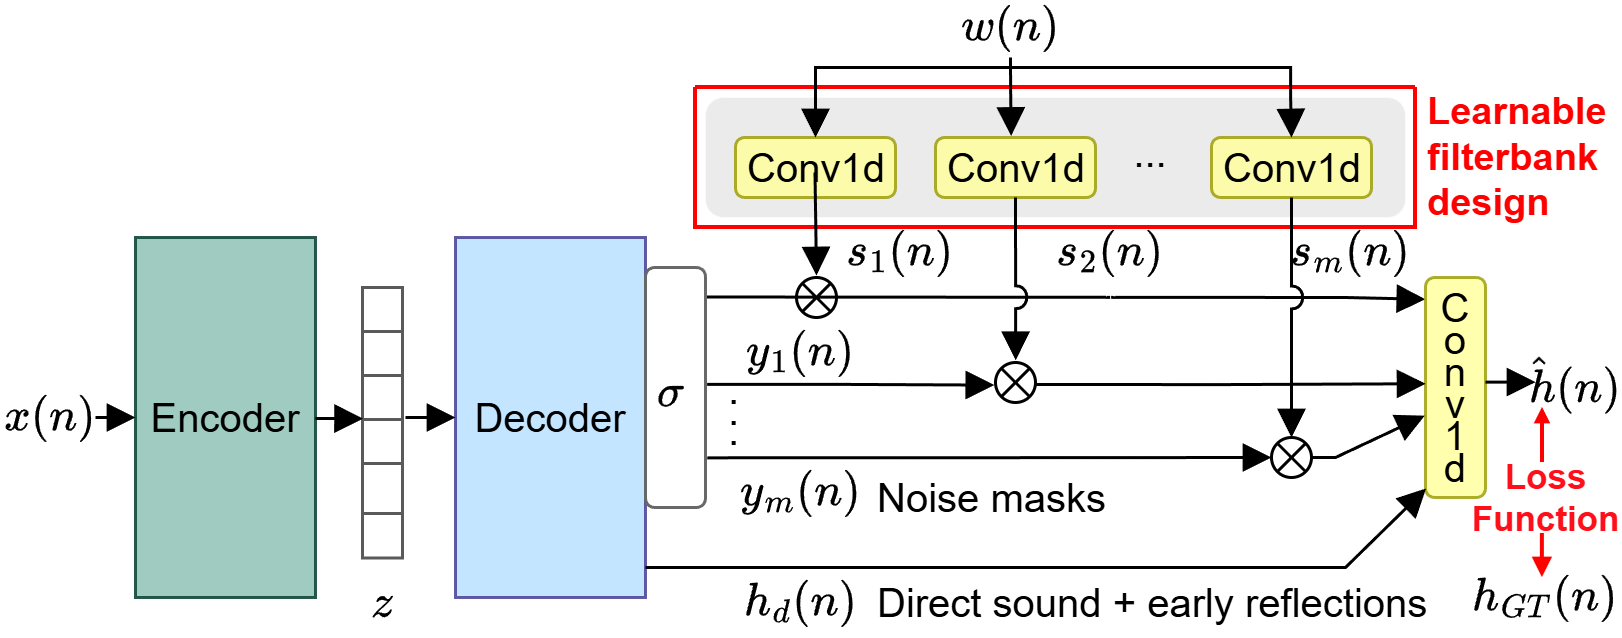
\includegraphics[width=\linewidth]{modified_FiNs.png}
    \caption{FiNS architecture and our key modifications (highlighted in red). Adapted from \cite{steinmetz2021filtered}.}
    \label{fig:arch2}
\end{figure}
 
\subsection{Modified Filterbank Architectures}
 
We investigated three alternative filterbanks: adapted octave filters, third-octave filters, and mel-scale filters. The following two approaches demonstrate superior performance:
 
%VORHER:
%\textbf{Adapted Octave Filters:} We develop data-driven filter optimization based on comprehensive statistical analysis of 11,500 real RIRs from our combined dataset. The analysis pipeline processes each RIR through 2048-sample FFT windows with 50\% overlap, computing averaged magnitude spectra and identifying significant spectral peaks using scipy.signal.find\_peaks with 3dB prominence thresholding. Statistical aggregation across the entire dataset reveals optimal frequency boundaries that reduce spectral overlap by 12\% compared to standard octave spacing while maintaining the 10-filter configuration. The adapted boundaries use the standard octave formula $f_l = f_c/2^{1/2}$ and $f_u = f_c \cdot 2^{1/2}$ but with empirically optimized center frequencies $f_c$ derived from dataset characteristics.
 
\textbf{Adapted Octave Filters:} In contrast to standard FiNS, which initializes learnable filterbanks with uniform octave spacing, we propose a data-driven initialization based on a statistical analysis of 11,500 real RIRs. To determine the initial center frequencies $f_c$, we process each RIR using 2048-sample FFT windows (50\% overlap) and identify significant spectral peaks via 3dB prominence thresholding. By aggregating these peaks, we derive empirically optimized values for $f_c$ that reduce initial spectral overlap by 12\% compared to standard spacing while maintaining the 10-filter configuration. Although the filter boundaries still follow the octave formula ($f_l = f_c/2^{1/2}$ and $f_u = f_c \cdot 2^{1/2}$), this initialization of $f_c$ provides a more informed starting point while preserving the adaptive capacity of the learnable architecture.
 
%\textbf{Adapted Octave Filters:} In contrast to standard FiNS implementation which initializes learnable filterbanks with uniform octave spacing, we propose a data-driven initialization approach based on comprehensive statistical analysis of 11,500 real RIRs from our combined dataset. The analysis pipeline processes each RIR through 2048-sample FFT windows with 50\% overlap, computing averaged magnitude spectra and identifying significant spectral peaks using scipy.signal.find\_peaks with 3dB prominence thresholding. Statistical aggregation reveals optimal frequency boundaries that reduce initial spectral overlap by 12\% compared to standard octave spacing while maintaining the 10-filter configuration. The adapted boundaries use the octave formula $f_l = f_c/2^{1/2}$ and $f_u = f_c \cdot 2^{1/2}$ but with empirically optimized initial center frequencies $f_c$ derived from dataset characteristics, providing a more informed starting point while preserving the adaptive capacity of the learnable architecture.
 
\textbf{Third-Octave Filters:} Implementation follows IEC 61260 \cite{IEC61260-2:2016} standard with 30 bands covering 25Hz-20kHz. Center frequencies are computed as $f_c[n] = 1000 \text{ Hz} \cdot 2^{n/3}$, where n ranges from -16 to +13, providing 3× higher spectral resolution with frequency progression factor $2^{1/3} \approx 1.26$ instead of 2.
 
All filterbanks employ FIR filters of order 1023 implemented as 1D convolutions with trainable coefficients. Following \cite{steinmetz2021filtered}, octave-bandpass initialization is used rather than standard Kaiming initialization to ensure proper convergence.
 
 
\subsection{Modified Loss Functions: MSTFT+EDR}
 
The original FiNS model employs an MSTFT loss, which combines spectral log-magnitude loss with spectral convergence. While effective for general spectral matching, the spectral convergence component lacks explicit modeling of the characteristic exponential energy decay patterns essential to room acoustics. We develop a combined approach that retains the fine-detail spectral log-magnitude component while replacing spectral convergence with EDR modeling:
\begin{equation}
L_{total} = \lambda_{MSTFT} L_{MSTFT} + \lambda_{EDR} L_{EDR},
\end{equation}
where $\lambda_{MSTFT}$ and $\lambda_{EDR}$ are weighting coefficients that balance the two loss components. The MSTFT component employs four different window sizes (64, 512, 2048, 8192 samples) to capture temporal and spectral characteristics across multiple resolutions, with spectral log-magnitude loss:
\begin{equation}
L_{MSTFT}(\hat{h}, h) = \frac{1}{N}| \log(|STFT(h)|) - \log(|STFT(\hat{h})|) |_1,
\end{equation}
where $\hat{h}$ is the estimated RIR, $h$ is the ground truth RIR, $N$ is the number of STFT frames, $|STFT(\cdot)|$ denotes the magnitude spectrogram, and $|\cdot|_1$ represents the L1 norm.
 
The EDR component models frequency-dependent energy decay across nine octave bands (16Hz-4kHz), following \cite{ratnarajah2023towards}:
\begin{equation}
EDR(r, t, b_k) = \sum_{\tau=t}^T |H(r, \tau, k)|^2,
\end{equation}
\begin{equation}
L_{EDR} = \mathbb{E}_{b_k}[(EDR(\hat{h}, t, b_k) - EDR(h, t, b_k))^2],
\end{equation}
where $H(r, \tau, k)$ represents the $k$-th frequency bin of the STFT at time $\tau$ for RIR $r$, $T$ the total duration, $b_k$ the $k$-th frequency band, and $\mathbb{E}[\cdot]$ the expectation operator over frequency bands.
 
%This formulation captures the characteristic exponential energy decay in room acoustics while maintaining frequency-specific modeling, essential for realistic reverberation synthesis. We evaluate EDR computation with three FFT sizes (1024, 2048, and 4096 samples; hereafter 1k, 2k, 4k samples) to optimize the time-frequency resolution trade-off: larger FFTs provide superior frequency resolution critical for low-frequency accuracy, while smaller FFTs maintain temporal precision for transient modeling. Weighting factors $\lambda_{\text{MSTFT}} = 1$ and $\lambda_{\text{EDR}} = 200$ were empirically determined to balance the scale differences between loss terms, ensuring comparable gradient magnitudes for both objectives during optimization.
 
This formulation captures the characteristic exponential energy decay in room acoustics while maintaining frequency-specific modeling, essential for realistic reverberation synthesis. We systematically evaluate EDR computation with three FFT sizes (1024, 2048, 4096 samples, hereafter 1k, 2k, 4k) to optimize the time-frequency resolution trade-off. Larger FFTs provide superior frequency resolution critical for low-frequency accuracy, while smaller FFTs maintain temporal precision important for transient modeling. Weighting factors $\lambda_{MSTFT} = 1$ and $\lambda_{EDR} = 200$ were empirically determined to balance the inherent scale differences between loss terms, ensuring comparable gradient magnitudes.
 
\begin{figure*}[htbp]
    \centering
    \renewcommand{\subfigtopskip}{0pt}       % Distance before subfigure
    \renewcommand{\subfigcapskip}{0.1cm}      % Distance between subfigure and caption
    \renewcommand{\subfigbottomskip}{-0.2cm}   % Distance after subfigure (incl. caption)
    
    \subfigure[Filter-based Models]{
        
\includegraphics[width=0.45\textwidth, trim=0 15 0 25, clip=TRUE]{filter_models_radar_chart.pdf}
        \label{fig:filter_models_radar_chart}
    }
    \hspace{1cm}
    \subfigure[MSTFT+EDR Models]{
        
\includegraphics[width=0.45\textwidth,, trim=0 15 0 25, clip=TRUE]{mstft_edr_plus_fins_radar_chart.pdf}
        \label{fig:mstft_edr_plus_fins_radar_chart}
    }
        
    \caption{Radar plots for performance comparison of (a) filter-based models and (b) MSTFT+EDR models. Values are normalized where 1.0 represents the best performing model for each metric, enabling direct visual comparison across different measurement scales and units.}
    \label{fig:radar-all}
\end{figure*}
 
 
\begin{table}[!t]
\centering
\caption{T60 and DRR Performance}
\vspace{-0.2cm}
\label{tab:t60_drr_results}
\resizebox{\columnwidth}{!}{%
\begin{tabular}{|l|ccc|ccc|}
\hline
\textbf{Model} & \multicolumn{3}{c|}{\textbf{T60}} & \multicolumn{3}{c|}{\textbf{DRR}} \\
\cline{2-7}
 & Bias $\rightarrow$ 0 & MSE (s) $\downarrow$ & $\rho$ $\uparrow$ & Bias $\rightarrow$ 0 & MSE (dB) $\downarrow$ & $\rho$ $\uparrow$ \\
\hline
FiNS Baseline    & 0.018 & 0.0047 & 0.955 & -1.61 & 26.56 & 0.742 \\
Adapted Octave   & \textbf{-0.003} & \textbf{0.0038} & 0.961 & -1.67 & 24.14 & 0.768 \\
Third-Octave     & 0.006 & 0.0039 & 0.960 & -1.55 & 27.90 & 0.715 \\
MSTFT+EDR 1k     & 0.034 & 0.0054 & 0.957 & -0.98 & \textbf{22.39} & \textbf{0.769} \\
MSTFT+EDR 2k     & -0.008 & 0.0045 & 0.954 & \textbf{0.72} & 23.24 & 0.748 \\
MSTFT+EDR 4k     & 0.011 & \textbf{0.0038} & \textbf{0.962} & 1.01 & 23.53 & 0.751 \\
\hline
\end{tabular}
}
\end{table}
 
\begin{table}[!htbp]
\centering
\caption{MSTFT Loss and Peak Similarity Performance}
\vspace{-0.2cm}
\label{tab:spectral_results}
\footnotesize
\makebox[\columnwidth]{%
\begin{tabular}{|l|c|cc|}
\hline
\textbf{Model} & \textbf{MSTFT} & \multicolumn{2}{c|}{\textbf{Peak Similarity}} \\
\cline{3-4}
 & Loss $\downarrow$ & Weighted $\uparrow$ & Unweighted $\uparrow$ \\
\hline
FiNS Baseline & 2.286 & 0.636 & 0.753 \\
Adapted Octave & 1.740 & 0.740 & 0.857 \\
Third-Octave & 1.838 & 0.712 & 0.833 \\
MSTFT+EDR 1k & 1.511 & 0.796 & 0.916 \\
MSTFT+EDR 2k & 1.369 & \textbf{0.797} & \textbf{0.926} \\
MSTFT+EDR 4k & \textbf{1.341} & 0.771 & 0.915 \\
\hline
\end{tabular}
}
\end{table}
 
\subsection{Model Training and Results}
 
Models were trained for 1500 epochs, AdamW optimizer, learning rate 5.5$\times$10$^{-5}$ with 0.8 decay every 80 epochs, batch size 32, gradient clipping (norm=5), 60/20/20 split ensuring proportional representation from all source datasets.
 
 
\begin{table}[!htbp]
\centering
\caption{Model Robustness: Standard Deviations Across Datasets}
\vspace{-0.2cm}
\label{tab:robustness}
\resizebox{\columnwidth}{!}{
\begin{tabular}{|l|c|c|c|c|c|c|}
\hline
\multirow{\textbf{Model}} & \multicolumn{3}{c|}{\textbf{T60}} & \textbf{MSTFT} & \multicolumn{2}{c|}{\textbf{Peak Similarity}} \\
\cline{2-7}
 & \textbf{Bias $\sigma$} & \textbf{MSE $\sigma$} & \textbf{$\rho$ $\sigma$} & \textbf{Loss $\sigma$} & \textbf{Wtd $\sigma$} & \textbf{Unwtd $\sigma$} \\
 & $\downarrow$ & $\downarrow$ & $\downarrow$ & $\downarrow$ & $\downarrow$ & $\downarrow$ \\
\hline
FiNS Baseline & 0.027 & 0.010 & 0.266 & 0.846 & 0.179 & 0.188 \\
Adapted Octave & 0.025 & 0.012 & 0.271 & 0.563 & 0.152 & 0.184 \\
Third-Octave & 0.016 & 0.008 & 0.265 & 0.530 & 0.160 & 0.208 \\
MSTFT+EDR 1k & 0.019 & 0.009 & 0.356 & \textbf{0.293} & 0.121 & 0.170 \\
MSTFT+EDR 2k & 0.018 & \textbf{0.003} & 0.183 & 0.352 & \textbf{0.103} & \textbf{0.162} \\
MSTFT+EDR 4k & \textbf{0.011} & 0.004 & \textbf{0.163} & 0.299 & 0.126 & 0.167 \\
\hline
\end{tabular}}
\vspace{-0.2cm}
\end{table}
 
Our analysis focuses on six model configurations: FiNS Baseline, Adapted Octave, Third-Octave, MSTFT+EDR variants (1k, 2k, 4k), excluding poorly performing variants for clarity.  Tables \ref{tab:t60_drr_results} and \ref{tab:spectral_results} present comprehensive performance across all key metrics. The MSTFT+EDR models demonstrate superior performance across most measures, with the 2k variant achieving optimal balance between spectral accuracy and temporal modeling (see Figure~\ref{fig:mstft_edr_plus_fins_radar_chart}).
 
\textbf{Model Robustness.} Table \ref{tab:robustness} quantifies performance consistency across diverse acoustic environments through standard deviations of key metrics. MSTFT+EDR models demonstrate superior consistency, with the 1k variant showing 65\% lower MSTFT loss variability ($\sigma$=0.293 vs 0.846 baseline) and the 2k variant achieving the most stable T60 estimation. This indicates better generalization across diverse acoustic environments. In addition to the standard deviation, MSTFT+EDR models show dramatically improved worst-case performance. The 1k variant reduces MSTFT loss range by 71\% and peak similarity range by ~40\%, while the 2k variant achieves the most stable T60 performance across challenging environments.
 
\textbf{Frequency-Dependent Energy Decay.} Table \ref{tab:edr_frequency} shows logarithmic EDR loss across nine frequency bands, revealing complementary strengths of different model configurations. Third-octave filters excel in low-end frequencies (16-32Hz), MSTFT+EDR 1k dominates mid-range (500Hz-1kHz), while MSTFT+EDR 4k achieves best high-frequency performance (2-4kHz), with 1k achieving best overall average EDR loss.

 
\begin{table*}[!t]
\centering
\caption{Frequency-Dependent Log EDR Loss Analysis (more negative values indicate lower EDR loss)}
\vspace{-0.2cm}
\label{tab:edr_frequency}
\footnotesize
\begin{tabular}{|l|c|c|c|c|c|c|c|c|c|c|}
\hline
%\small
\textbf{Model} & \textbf{16Hz $\downarrow$} & \textbf{32Hz $\downarrow$} & \textbf{63Hz $\downarrow$} & \textbf{125Hz $\downarrow$} & \textbf{250Hz $\downarrow$} & \textbf{500Hz $\downarrow$} & \textbf{1kHz $\downarrow$} & \textbf{2kHz $\downarrow$} & \textbf{4kHz $\downarrow$} & \textbf{Avg $\downarrow$} \\
\hline
FiNS Baseline & -1.72 & -1.84 & -2.13 & -2.50 & -3.24 & -3.37 & -3.35 & -3.56 & -3.81 & -2.84 \\
Adapted Octave & -1.78 & -1.85 & -2.18 & -2.66 & -3.41 & -3.48 & -3.44 & \textbf{-3.86} & -3.88 & -2.95 \\
Third-Octave & \textbf{-1.82} & \textbf{-1.92} & -2.13 & -2.37 & -3.22 & -3.29 & -3.39 & -3.54 & -3.57 & -2.81 \\
MSTFT+EDR 1k & -1.67 & -1.76 & \textbf{-2.42} & -2.90 & -3.46 & \textbf{-3.61} & \textbf{-3.78} & -3.83 & -4.00 & \textbf{-3.05} \\
MSTFT+EDR 2k & -1.69 & -1.89 & -2.27 & \textbf{-2.97} & -3.45 & -3.42 & -3.36 & -3.44 & -3.48 & -2.89 \\
MSTFT+EDR 4k & -1.81 & -1.89 & -2.35 & -2.79 & \textbf{-3.48} & -3.49 & -3.52 & \textbf{-3.86} & \textbf{-4.11} & -3.03 \\
\hline
\end{tabular}
\vspace{-0.1cm}
\end{table*}
 
 
\section{Discussion}
 
\textbf{Evaluation Metrics.} Peak similarity has proven effective in quantifying frequency peak accuracy. The weighted variant in particular revealed systematic shifts of dominant low-frequency peaks in FiNS-generated RIRs, shifts that are not specifically captured by MSTFT-based metrics. Given the perceptual relevance of this frequency range \cite{fazenda2015}, these shifts may contribute to audible differences between synthetic and measured RIRs reported in prior listening tests \cite{steinmetz2021filtered}, representing an overlooked limitation in FiNS-based RIR generation. This finding illustrates the broader value of multi-metric evaluation: limitations invisible to one metric can become apparent through another, with radar plots (Figure~\ref{fig:radar-all}) making such trade-offs comparable across models.
 
\textbf{Modified Filterbank Architectures.} Among filter-based approaches, the adapted octave filter improves T60 estimation and overall spectral accuracy, showing informed initialization outperforms uniform spacing. Third-octave filters outperform the baseline in most metrics and surpass the adapted variant in low-frequency EDR (Table~\ref{tab:edr_frequency}), yet despite their higher band resolution the adapted variant remains stronger overall.
 
% The MSTFT+EDR approach achieved 41\% MSTFT loss reduction (1.341 vs 2.286 baseline), 25\% peak similarity improvement (0.926 vs 0.753), superior energy decay modeling (-3.05 average EDR loss), and 65\% reduction in performance variability across the choosen datasets. 
 
\textbf{Modified Loss Function.} The superior performance of MSTFT+\linebreak[2]EDR models across all metrics validates that augmenting the MSTFT loss with an EDR component ensures a more precise capture of the underlying room acoustic properties. This combined approach not only improves overall performance but excels even in metrics primarily associated with individual components, achieving better MSTFT loss than baseline while providing superior energy decay modeling. This effectiveness is likely due to the EDR component explicitly incorporating the exponential energy decay inherent to room acoustics, whereas spectral convergence treats spectral evolution without such a physical inductive bias.
 
\textbf{Model Robustness.}
MSTFT+\-EDR models show higher consistency across diverse acoustic environments, with 65\% lower MSTFT loss variability than the baseline. This robustness is crucial for deployment where models must perform reliably across acoustic conditions. Dataset-specific analysis identifies Palimpsest (historic maritime structures) and C4DM (large university halls) as particularly challenging environments, with a 25-35\% performance degradation compared to controlled environments, yet MSTFT+EDR models maintain superior relative performance even in these scenarios. 
 
\textbf{Comparison of approaches.} Our analysis reveals complementary frequency-specific strengths across model variants. Third-octave filters excel at very low frequencies (16--32 Hz), whereas MSTFT+EDR variants show superior performance in specific mid-to-high ranges depending on the FFT size: the 1k window dominates the 500--1000 Hz range, while the 4k window excels at 2--4 kHz. Larger FFT windows provide finer frequency resolution, which is particularly useful for resolving
narrowband structures, including low-frequency modes and detailed high-frequency spectral patterns, whereas smaller windows preserve temporal precision.
 
 
\section{Conclusion}
 
%Together with a representative dataset of diverse RIRs, our multi-metric approach allows automatic and convenient evaluation of RIRs. This may improve comparability between future models without requiring access to codebases that are often not publicly available, and may enable more energy-efficient evaluation by allowing reuse of published results instead of retraining competing approaches. Incorporating ten different metrics, our evaluation framework provides a detailed comparison by taking various aspects of blind room impulse response generation into account. Moreover, the visual representation of these metrics in radar plots provides a convenient way to visually compare different RIR generation techniques, revealing metric trade-offs.

Our multi-metric approach, combined with a collection of diverse RIR datasets, enables convenient and standardized evaluation. This may improve comparability between future models without requiring access to codebases that are often not publicly available, and may enable more energy-efficient evaluation by allowing reuse of published results instead of retraining competing approaches. Incorporating ten metrics, our evaluation framework provides a detailed comparison by taking various aspects of blind room impulse response generation into account. Moreover, the visual representation of these metrics in radar plots provides a convenient way to compare methods while revealing metric trade-offs.

In our experiments, we effectively assessed architectural and loss function optimizations of FiNS, with insights likely transferable to future FiNS-based architectures. We showed that the combined MSTFT+EDR loss outperforms the original MSTFT-based FiNS setting, data-driven filterbank optimization surpasses theoretical designs, and systematic FFT size evaluation reveals critical time-frequency resolution trade-offs. MSTFT+EDR 2k provides optimal overall balance, adapted octave filters excel for T60-critical applications, while MSTFT+EDR 4k excels in spectral accuracy.

Current limitations include fixed 1-second length and single-channel restriction. Future directions include architecture hybridization and multi-channel extension. Furthermore, formal perceptual evaluation through listening tests could validate the objective improvements, as well as the perceptual relevance of our peak similarity metric and framework.
 
% , achieving 41\% MSTFT loss reduction (1.341 vs 2.286 baseline), 25\% peak similarity improvement (0.926 vs 0.753), superior energy decay modeling (-3.05 average EDR loss), and 65\% reduction in performance variability across the choosen datasets
% This research establishes enhanced foundations for neural acoustic modeling with practical guidance for application-specific optimization, significantly reducing the perceptual gap between synthetic and measured room responses.
 
%\FloatBarrier
%\vspace*{\fill}
%\clearpage
\bibliographystyle{IEEEbib}
\bibliography{myLiteratureFINs,myLiteratureFINs2,myLiteratureWEIRD,references,refs.bib}
 
\end{document}